\subsection{Buttons and button design}
\label{GUI:buttons}

To make the overall consistency and usability better there were made some button guidelines. These were made to be used in the \giraf[] GUI library and thereby in the hole \giraf[] system including the launcher.

These guidelines included colors the buttons should have. The edge of the button should be a dark brown and the inner should be yellow and hereby the buttons are using the commen \giraf[] colors. Buttons should also have round corners if they are clickable and if they for some reason are not they should be squared. This can be seen in \autoref{fig:buttons}.

\begin{figure}[h!]
	\centering
	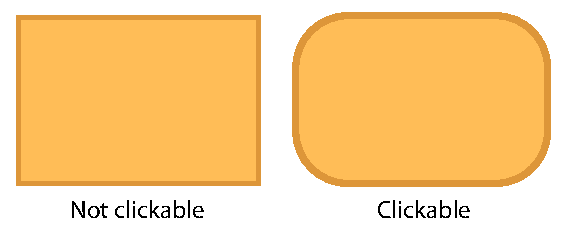
\includegraphics[scale=0.6]{gfx/buttons.pdf}
	\caption{Button illustration}
	\label{fig:buttons}
\end{figure}


\todo{Should this section be here?}